\documentclass[preview]{standalone}

\usepackage{tikz}
\usetikzlibrary{arrows, calc, patterns, decorations.pathmorphing, decorations.markings}

\begin{document}
	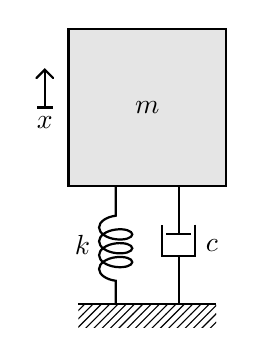
\begin{tikzpicture}[every node/.style={draw, outer sep=0pt, thick}]
	\tikzstyle{spring}=[
		thick,
		decorate,
		decoration={
			coil,
			amplitude = 6pt,
			pre length=0.3cm,
			post length=0.3cm,
			segment length=5
		}
	]
	\tikzstyle{damper}=[
		thick,
		decorate,
		decoration={
			markings,  
			mark connection node=dmp,
			mark=at position 0.5 with
			{
				\node (dmp) [thick, inner sep=0pt, transform shape, rotate=-90, minimum width=12pt, minimum height=8pt,draw=none] {};
				\draw [thick] ($(dmp.north east)+(3.5pt,0)$) -- (dmp.south east) -- (dmp.south west) -- ($(dmp.north west)+(3.5pt,0)$);
				\draw [thick] ($(dmp.north)+(0,-4.5pt)$) -- ($(dmp.north)+(0,4.5pt)$);
			}
		}
	]
	\tikzstyle{ground}=[
		fill,
		pattern=north east lines,
		draw=none,
		minimum width=0.75cm,
		minimum height=0.3cm
	]
	
	\node (M) [minimum width=2cm, minimum height=2cm, fill=black, fill opacity=0.1, text opacity=1] {$m$};
	
	\node (ground) at (M.south) [ground, yshift=-1.5cm, minimum width = 1.75cm, anchor=north] {};
	\draw [thick] (ground.north west) -- (ground.north east);
	
	\draw [spring] ($(ground.north)+(-0.4cm,0)$) -- ($(M.south)+(-0.4cm,0)$)
		node[midway, xshift=-12pt, draw=none]{$k$};
	\draw [damper] ($(ground.north)+(0.4cm,0)$) -- ($(M.south)+(0.4cm,0)$)
		node[midway, xshift=12pt, draw=none]{$c$};
	
	\draw [thick] (M.west) ++(-0.2cm,0cm) -- +(-0.2cm,0cm)
		node[midway, below, draw=none]{$x$};
	\draw [thick, -angle 90] (M.west) ++(-0.3cm,0cm) -- +(0,0.5cm);
	\end{tikzpicture}
\end{document}